\chapter{Introduction} \label{ch:Introduction}
Given functions $g(x)$ and $k(x,t)$, the \textit{Fredholm equation of the first kind} is
\begin{equation}
g(x) = \int_a^b k(x,t)f(t)\:dt,
\label{eq:FIE}
\end{equation}
where the function $f(t)$ is unknown \cite[p.~218]{DebnathMikusinski2005}. If the kernel $k(x,t)$ is of the form $k(x,t) = k(x-t)$ and the limits of integration are infinite, then the integral equation represents the continuous convolution $g(x) = (k * f)(x)$. In general, convolution is a smoothing operation: if $k(x-t)$ is integrable and $f(t)$ is bounded and locally integrable, then $g(x)$ is a continuous function \cite{DebnathMikusinski2005}. In particular, if $k(x-t)$ and $f(t)$ are at least piecewise smooth and bounded, the resulting convolution $g(x)$ is continuous. \par
If convolution is considered a smoothing operation, then finding $f(t)$ such that $g(x) = (k * f)(x)$, given $g(x)$ and $k(x-t)$, could be considered a ``sharpening" operation. For instance, consider the kernel $k(t) = \exp(-200(t-\frac{1}{2})^2)$ and the piecewise-smooth function $f(t)$ defined as:
\begin{equation}
f(t) = \begin{cases}
\sin\left(8\pi{t}\right), & 0 < t \leq \frac{1}{4} \\
0, & \frac{1}{4} < t \leq \frac{1}{3} \\
24\left(t-\frac{1}{3}\right), & \frac{1}{3} < t \leq \frac{3}{8} \\
1, & \frac{3}{8} < t \leq \frac{5}{8} \\
-24\left(t-\frac{2}{3}\right), & \frac{5}{8} < t \leq \frac{2}{3} \\
0, & \frac{2}{3} < t \leq \frac{3}{4} \\
\sin\left(8\pi\left(t-\frac{3}{4}\right)\right), & \frac{3}{4} < t \leq 1
\end{cases}.
\label{eq:Test Function 2}
\end{equation}
The kernel $k(x-t)$ is smooth and bounded on $[0,1]$, and the function $f(t)$ is 1-periodic and bounded. Plots of $f(t)$ and $k(t)$ are shown in Figure \ref{FunctionKernelPlot}. \par
The kernel $k(t) = \exp(-200(t-\frac{1}{2})^2)$ is an example of a Gaussian kernel. The form of a Gaussian kernel comes from the probability density function of the Gaussian distribution,
\begin{equation}
p(t) = \frac{1}{\sqrt{2\pi\noiseSD^2}}\exp\left(\frac{-(t-\mu)^2}{2\noiseSD^2}\right),
\label{eq:Gaussian kernel}
\end{equation}
where $\mu$ is the mean and $\noiseSD^2$ is the variance. The mean is the center of the Gaussian distribution, as well as the abscissa of the absolute maximum of the probability density function $p(t)$. The variance $\noiseSD^2$ is a measure of dispersion of the distribution; as $\noiseSD^2$ increases, the width of the graph of $p(t)$ increases. The standard deviation $\noiseSD$ is also a measure of dispersion. The scale factor $1/\sqrt{2\pi\noiseSD^2}$ ensures that $\int_{\mathbb{R}} p(t) \: dt = 1$, an essential property of a continuous probability distribution defined on the entire real line. For Gaussian kernels, however, this scale factor may be dropped since having a unitary integral is not required of kernels in general.  For the Gaussian kernel example $k(t) = \exp(-200(t-\frac{1}{2})^2)$, the mean is 1/2 and $-1/2\noiseSD^2 = -200$ implies that $\noiseSD = 1/20$. For the sake of convenience, the width parameter of a Gaussian kernel will refer to the value of $1/2\noiseSD^2$. Figure \ref{GaussianDistributions} illustrates the relationship between variance and width of the Gaussian distribution. As a last remark, we use the kernel $k(x,t)$, function $f(t)$ \eqref{eq:Test Function 2}, and resulting function $g(x)$ repeatedly for the numerical examples.

\begin{figure}
	\centerline{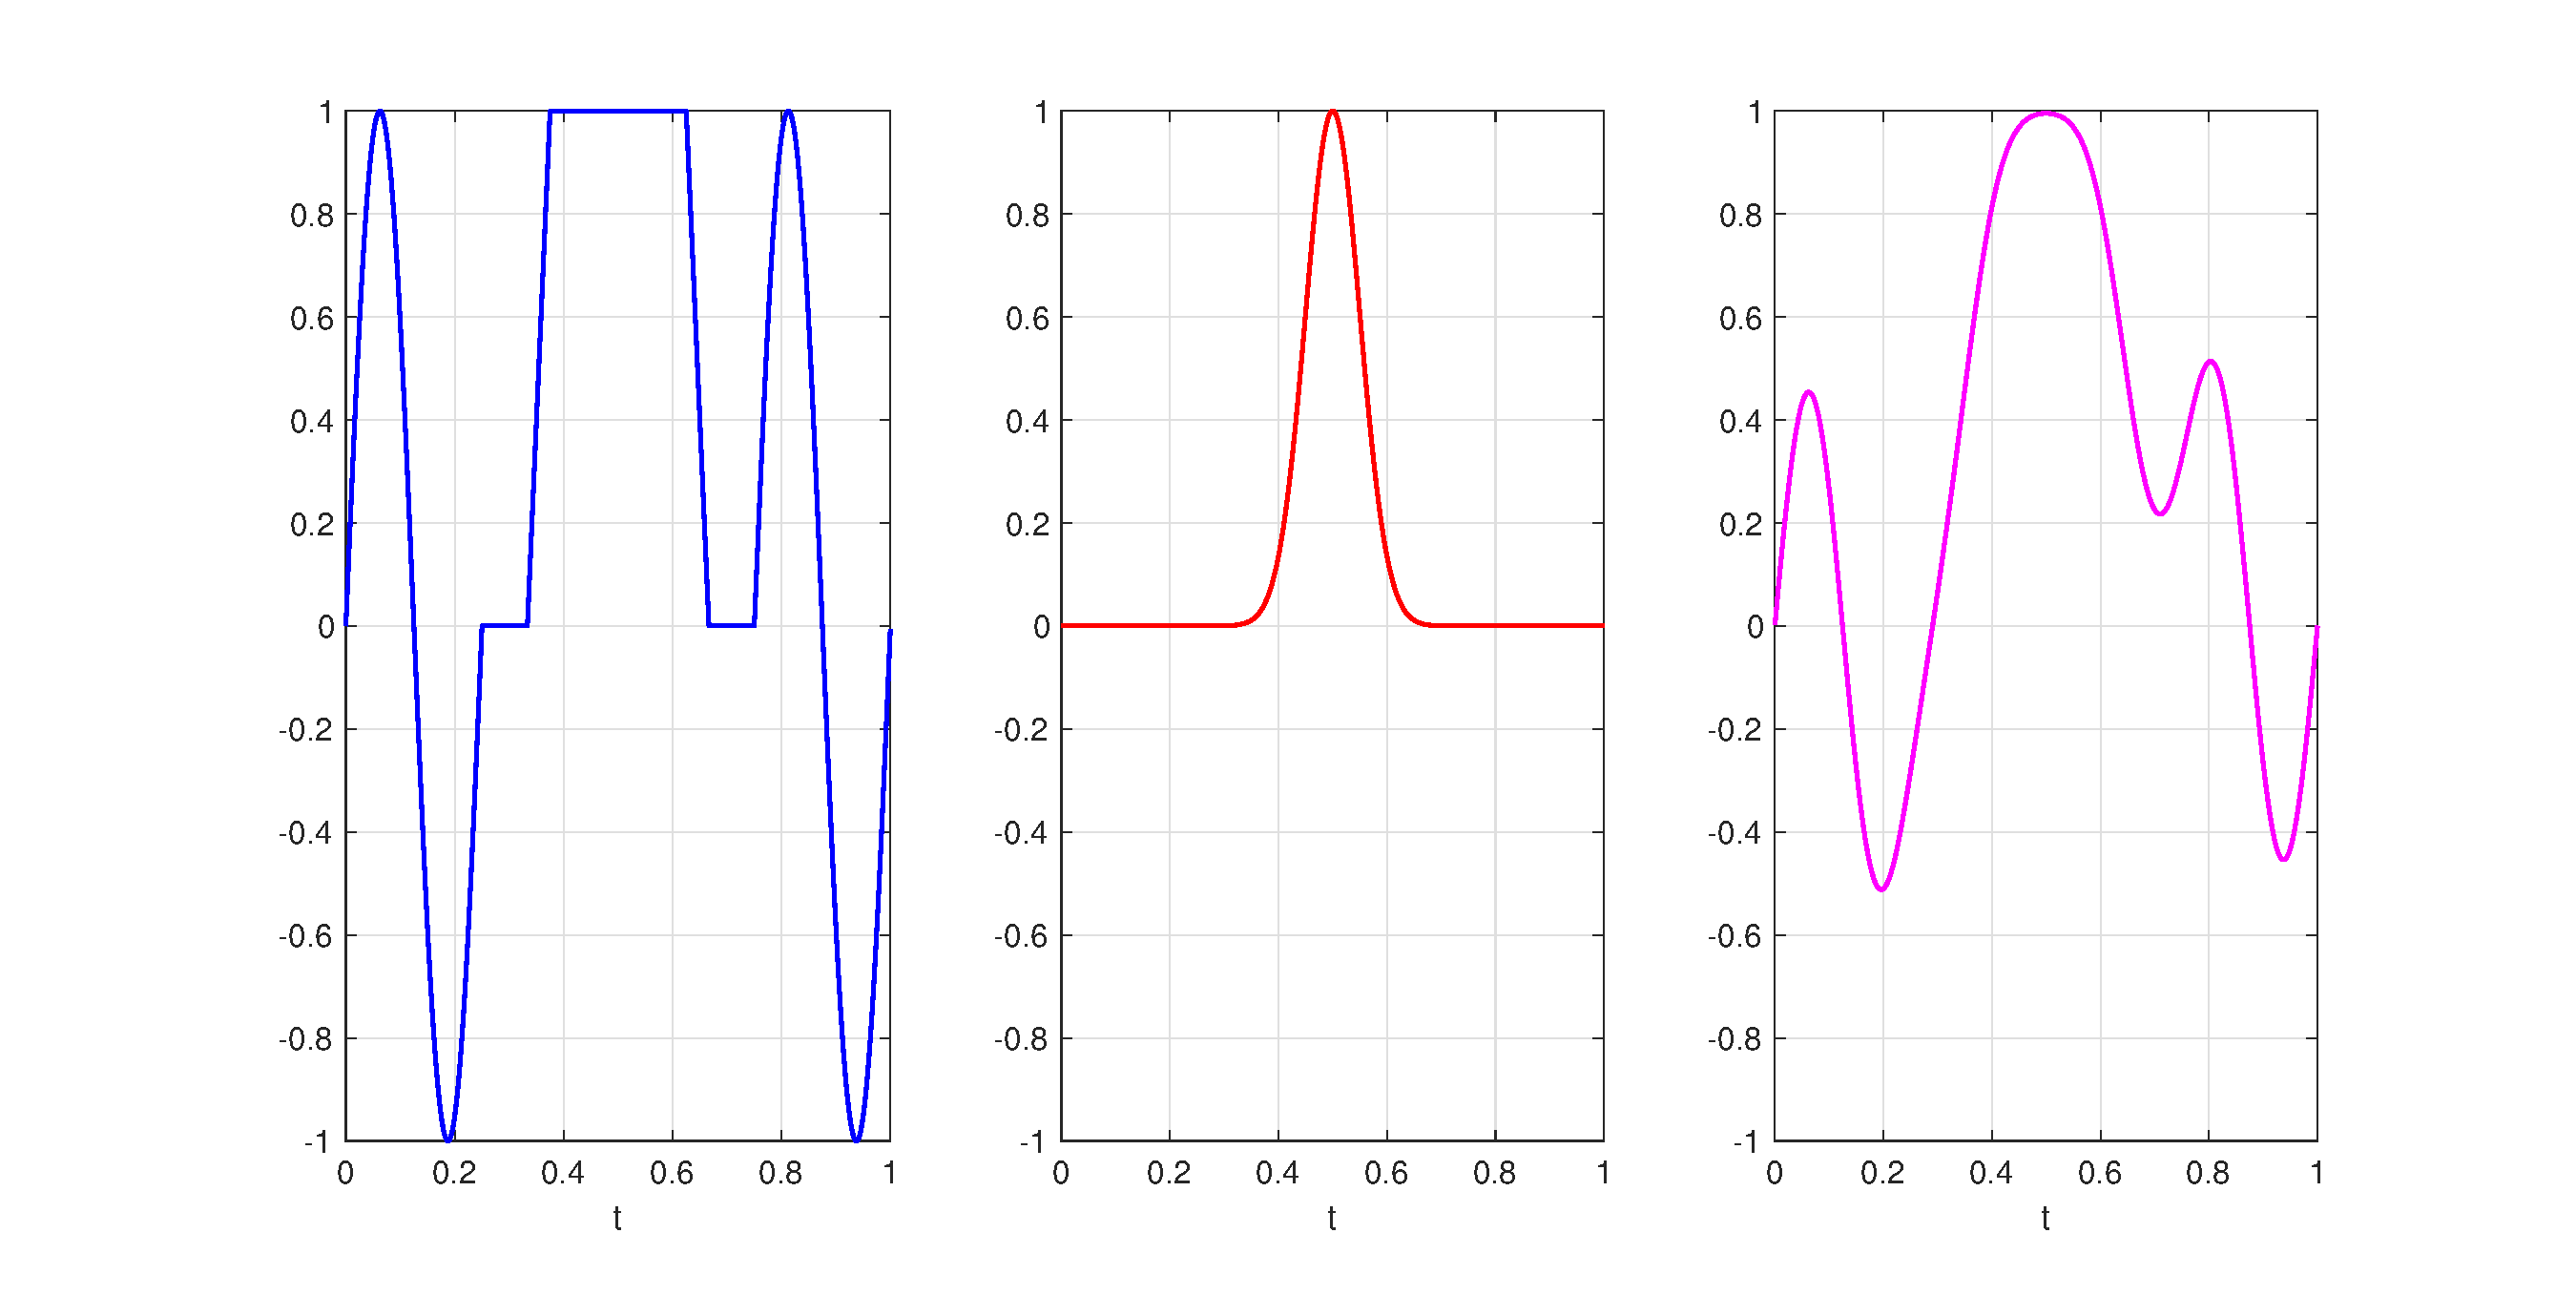
\includegraphics[scale=0.4]{Figures/FunctionKernelPlot.eps}}
\caption{Left: The graphs of the piecewise-smooth function $f(t)$ given by \eqref{eq:Test Function 2}. Center: The Gaussian kernel $k(t)$. Right: The function $g(x) = (f * g)(x)$. Notice that the corners of the graph of $f(t)$ have been smoothed over as a result of the convolution.}
\label{FunctionKernelPlot}
\end{figure}

\begin{figure}
	\centerline{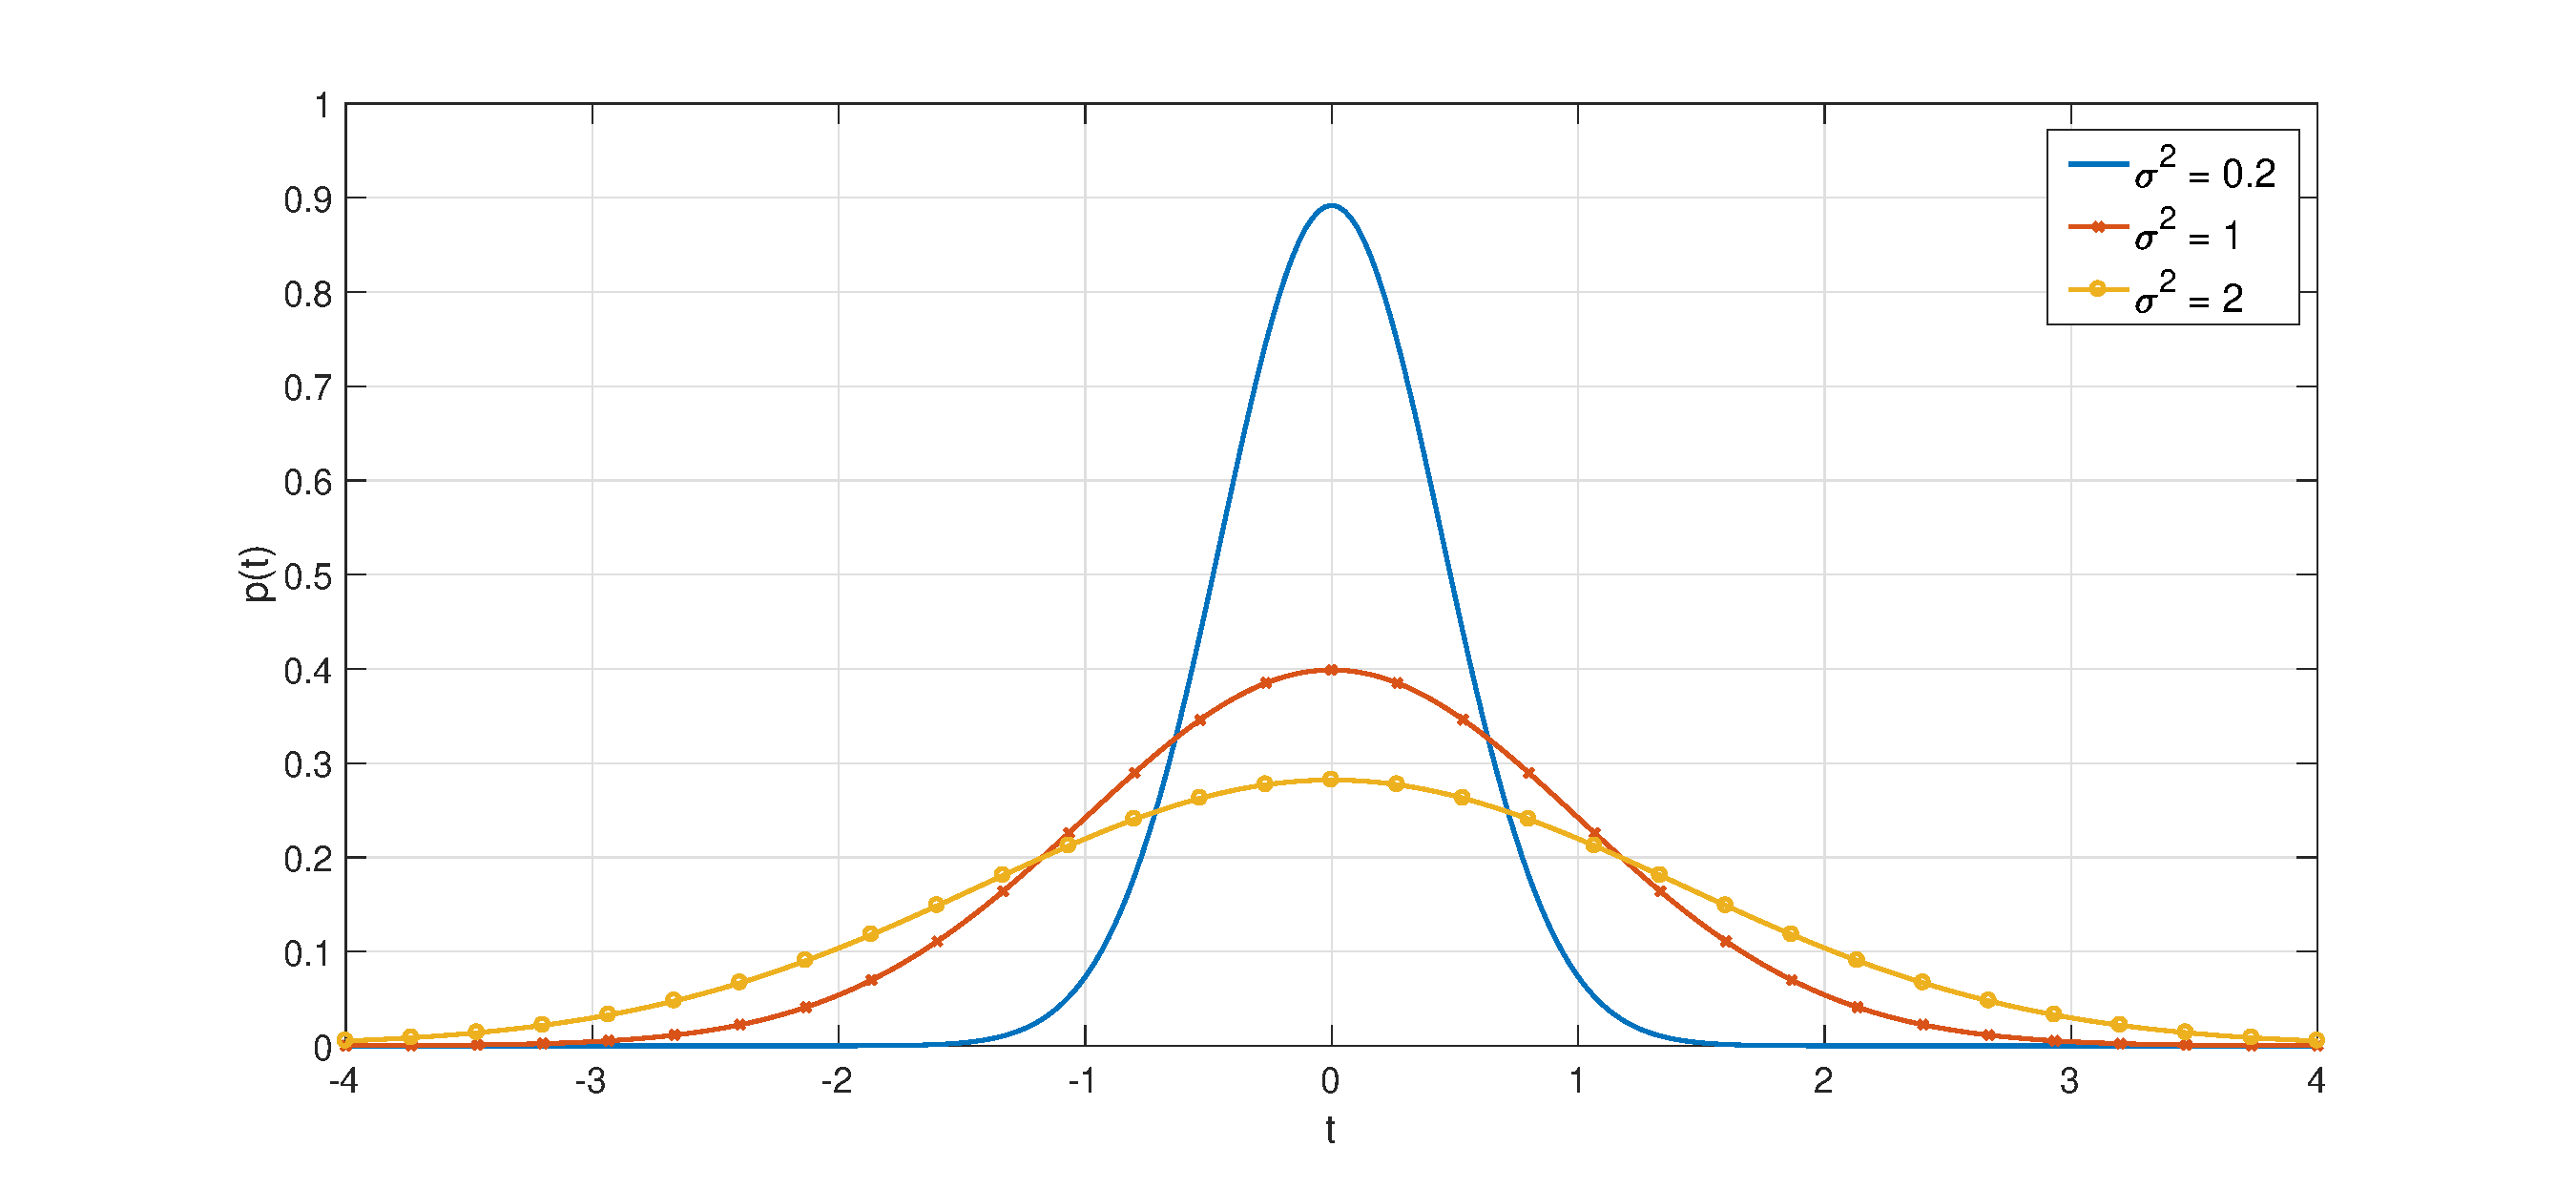
\includegraphics[scale=0.4]{Figures/GaussianDistributions.eps}}
\caption{Gaussian distributions for difference values of variance $\noiseSD^2$, all centered at the origin ($\mu = 0$). As $\noiseSD^2$ increases, the width of the distribution increases.}
\label{GaussianDistributions}
\end{figure}

If the kernel $k(x-t)$ in \eqref{eq:FIE} has compact support, then the limits of integration can be expressed as finite values that depend upon the support of $k(x-t)$. For example, if the support of $k(x-t)$ is $[\alpha_k,\beta_k]$, then \eqref{eq:FIE} becomes
\begin{equation}
\label{eq:FIE 2}
g(x) = \int_{-\infty}^{\infty} k(x-t)f(t) ~dt = \int_{x-\beta_k}^{x-\alpha_k} k(x-t)f(t) ~dt.
\end{equation} 
More rigorously, if $k(x-t)$ is compactly supported and $f(t)$ is locally integrable, then $g(x) = (k*f)(x)$ exists and is continuous. Existence follows directly from the condition of local integrability, which means that $\int_a^b f(t) ~dt$ exists for every $-\infty < a < b < \infty$; the space of locally integrable functions is a subspace of $L^1(\mathbb{R})$ \cite[p.~63]{DebnathMikusinski2005}. In real-world applications, data is finite and in the context of \eqref{eq:FIE}, this means that information about $g(x)$ is only known over a finite interval. Suppose information about $g(x)$ is only known over the interval $[\alpha_g,\beta_g]$. Then using \eqref{eq:FIE 2}, $g(\alpha_g)$ and $g(\beta_g)$ are given by
\[g(\alpha_g) = \int_{\alpha_g-\beta_k}^{\alpha_g-\alpha_k} k(\alpha_g - t)f(t) ~dt, \quad g(\beta_g) = \int_{\beta_g - \beta_k}^{\beta_g - \alpha_k} k(\beta_g-t)f(t) ~dt.\]
Without loss of generality, suppose $[\alpha_k,\beta_k] = [-\frac{1}{2},\frac{1}{2}]$ and $[\alpha_g,\beta_g] = [0,1]$. Then $\alpha_g-\beta_k = -\frac{1}{2}$ and $\beta_g - \alpha_k = \frac{3}{2}$, meaning that the support of $f(t)$ affecting the given data about $g(x)$ is $[-\frac{1}{2},\frac{3}{2}]$. In other words, if a solution $f(t)$ is only desired over the support of $g(x)$, then boundary conditions must be imposed on $f(t)$ so that the corresponding discrete system will not be underdetermined; this is addressed in Chapter \ref{ch:Results}. \par 
To find a solution to the forward problem, which is the evaluation of $g(x) = (k * f)(x)$, a quadrature method can be used to find a numerical approximation to the convolution integral. In the discrete setting, (1) can be stated as
\begin{equation}
\gVec = \kMat\fVec,
\label{eq:Dis}
\end{equation}
where $\fVec$ and $\gVec$ are the vector discretization of $f(t)$ and $g(x)$, respectively, and $\kMat$ is a matrix representing the discrete convolution of $k(x,t)$ with $f(t)$. For example, suppose $k(x,t)$ is a zero-centered Gaussian kernel and the domain of integration in \eqref{eq:FIE} is $[0,1]$. Given some $x_j \in [0,1]$, the continuous forward problem is to evaluate
\[g(x_j) = \int_0^1 \exp\left(\frac{-(x_j - t)^2}{2\noiseSD^2}\right)f(t) \: dt.\]
If a left Riemann sum is used with $t_k = k/n$ for $k \in \{0,1,\ldots,n-1\}$, representing an equispaced discretization of $[0,1]$ using $n$ points, then
\[g(x_j) \approx \sum_{k=1}^n \frac{1}{n}\exp\left(\frac{-(x_j - t_k)^2}{2\noiseSD^2}\right)f(t_j).\]
For approximations to $g(x)$ at the same points that make up the equispaced discretization of $[0,1]$, i.e. at the points $x_j = j/n$ for $j \in \{0,1,\ldots,n-1\}$, then \eqref{eq:Dis} is exactly the system that provides these approximations with $\fVec = [f(t_0),f(t_1),\ldots,f(t_{n-1})]$, $\gVec = [g(x_0),g(x_1),\ldots,g(x_{n-1})]$, and the elements of $\kMat$ being
\[K_{j,k} = \frac{1}{n}\exp\left(\frac{-(j - k)^2}{2\noiseSD^2}\right), \quad 0 \leq j,k \leq n-1.\]
Note that taking the collocation and quadrature points as the same ensures that the matrix $\kMat$ is square. Changing the number of collocation points, or the quadrature method, can change $\kMat$ from square to rectangular; see Section \ref{sec:DFT}. \par
If the matrix $\kMat$ is nonsingular, then the solution to the inverse problem \eqref{eq:Dis} is $\fVec = \kMat^{-1}\gVec$. As with many linear systems, however, direct matrix inversion is discouraged and usually impractical since the matrix $\kMat$ can become increasingly ill-conditioned as the size of the system grows \cite[p.~2]{Vogel:2002}. Unfortunately, large systems are often necessary to adequately approximate the continuous problem, and so other methods of solving for $\fVec$ must be considered. \par
Before discussing the consequences of ill-conditioning, the concept of a well-posed problem will be introduced, which is due to Hadamard \cite{Hadamard1904}. Given an operator $A : \mathcal{H}_1 \rightarrow \mathcal{H}_2$, where $\mathcal{H}_1$ and $\mathcal{H}_1$ are Hilbert spaces, the equation $Af = g$ is said to be well-posed if
\begin{enumerate}
\item[(i)] for each $g \in \mathcal{H}_2$ there exists a solution $f \in \mathcal{H}_1$ to $Af = g$,
\item[(ii)] the solution $f$ is unique, and
\item[(iii)] if $Af_* = g_*$ and $Af = g$, then $f \rightarrow f_*$ whenever $g \rightarrow g_*$.
\end{enumerate}
In order, these conditions require that a solution exists, is unique, and is stable under perturbations in $g$. If one of these conditions is not met, then $Af = g$ is said to be an ill-posed problem. The discrete problem $\kMat\fVec = \gVec$ can be ill-posed under a number of circumstances: singularity of $\kMat$ violates conditions (i) and (ii), and a poor condition number of nonsingular $\kMat$ violates condition (iii). If the matrix $\kMat$ is rectangular, then $\kMat$ is singular and certainly (i) is violated.  \par 
A primary consequence of $\kMat$ being ill-conditioned relates to the accuracy of the vector $\gVec$. If $\gVec$ contains errors, as is often the case in practical applications, the errors are amplified during the multiplication $\kMat^{-1}\gVec$ since $\kMat$ is ill-conditioned. As a result, the obtained solution $\fVec$ will suffer from a large amount error; $\fVec$ is thus sensitive to errors in $\gVec$. For this consideration, the following system will be the assumed model
\begin{equation}
\gnoiseVec = \kMat\fVec + \noiseVec,
\label{eq:DisNoise}
\end{equation}
where $\noiseVec$ is a vector that represents any errors in $\gVec$ (this is equivalent to the statement $\gnoiseVec = \gVec + \noiseVec$). For further simplicity, assume that $\noiseVec \sim \mathcal{N}(\zeroVec,\noiseSD^2I)$, where $\zeroVec$ is the zero vector of length $n$ and $I$ is the $n \times n$ identity matrix. In other words, the error vector $\noiseVec$ is a realization of an $n$-dimension Gaussian random variable with mean zero and variance $\noiseSD^2$. 

\section{Main contributions and overview}
The contributions of this research are twofold. First, the regularization parameter estimation functions pertaining to the unbiased predictive risk estimator, the generalized cross validation method, and the discrepancy principle are formulated from the perspective of the discrete Fourier and cosine transform. In other words, the functions use the discrete Fourier and cosine transform components as opposed to singular values. Second, the effects of downsampling on parameter estimation are evaluated both qualitatively and quantitatively. The qualitative characteristics of these effects can be analyzed by using empirical statistics obtained from numerical examples in conjunction with multiple realizations of noise (see Section \ref{sec:Downsampling and white noise}). The quantitative characteristics are currently incomplete and are one of the goals of future research. \par
Chapter \ref{ch:Analytical tools} will present tools and ideas that are commonly used for the solution of inverse problems. Two primary tools, the discrete  Fourier and cosine transforms, are discussed in Section \ref{sec:Discrete trig. transforms}. The numerical examples considered in conjunction with these transforms are explained in Chapter \ref{ch:Results}. \par 
Since the assumed model problem \eqref{eq:DisNoise} contains random noise, a discussion of statistical results is included in Chapter \ref{ch:Stats}. The statistical results pertain not only to the nature of the noise under various transformations but also serve as a motivation for the parameter estimation methods contained in Chapter \ref{ch:Parameter estimation methods}. In addition to introducing the parameter estimation methods, Chapter \ref{ch:Parameter estimation methods} also presents new formulations of the parameter estimation functions which are based on the DFT and DCT. Versions of the the parameter estimation functions which assume the availability multiple data sets are available are also provided.  \par  
A two-dimension problem is considered in Chapter \ref{ch:Results}, which presents some of the interesting extensions of the one-dimensional concepts. Lastly, some conclusions and observations are made in Chapter \ref{ch:Conclusion}. The observations are used to motivate the goals of future work, which include consideration of three-dimensional numerical examples and quantitative descriptions of the effects of downsampling.
